\subsection{Finite Differences}\label{subsec:finite_differences}

In this section we will be looking into finite difference methods. Finite difference methods are a class of numerical methods for solving differential equations by approximating derivatives with finite differences. The basic idea is to replace the continuous derivatives in the differential equation with discrete approximations based on the values of the function at a set of grid points. We use finite differences only as a check to validate our low-P\'eclet number FEM results, so we will not be looking very deeply into this method. We will describe finite differences with a simple example, show how this leads to oscilations, and then show how to fix this using upwind methods. 

A lot of the theory is implemented automatically in the MethodOfLines.jl package.

\subsubsection{Central Finite Differences}
Finite differences uses a discretization of the domain. Say we want to discretize the domain $[a, b]$ into $N$ intervals, we can define the discretization as follows:
\begin{equation}
    x_i = a + i\Delta x, \quad i = 0, 1, \ldots, N,
\end{equation}
where $\Delta x = (b-a)/N$ is the spatial step size. Now our control vector $\mathbf{u}$ becomes:
\begin{equation}
    \mathbf{u}(t) = \begin{pmatrix}
        u(x_0, t) \\
        u(x_1, t) \\
        \vdots \\
        u(x_{N-1}, t) \\
        u(x_N, t)
    \end{pmatrix}
\end{equation}

Say we have the simple diffusion equation:
\begin{equation}
    \partial_t u = D \partial_{xx} u,
\end{equation}
where $D$ is the diffusion coefficient. With initial condition and boundary conditions:
\begin{equation}
    \begin{aligned}
        u(x, 0) &= u_0(x), \\
        u(a, t) &= g_a(t), \\
        u(b, t) &= g_b(t),
    \end{aligned}
\end{equation}

Now we can approximate the second derivative using finite differences. The second derivative can be approximated using the central difference scheme:
\begin{equation}
    \partial_{xx} u(x_i, t) \approx \frac{u(x_{i+1}, t) - 2u(x_i, t) + u(x_{i-1}, t)}{\Delta x^2}.
\end{equation}
for all $i = 1, 2, \ldots, N-1$. This leads to a semi-discrete system of ODEs:
\begin{equation}
    \partial_t \mathbf{u}(t) = D A \mathbf{u}(t),
\end{equation}
where $A$ is the matrix representing the finite difference approximation of the second derivative. The matrix $A$ is a tridiagonal matrix with the following structure:
\begin{equation}
    A = \frac{1}{\Delta x^2} \begin{pmatrix}
        -2 & 1 & 0 & \cdots & 0 \\
        1 & -2 & 1 & \cdots & 0 \\
        0 & 1 & -2 & \cdots & 0 \\
        \vdots & \vdots & \vdots & \ddots & 1 \\
        0 & 0 & 0 & 1 & -2
    \end{pmatrix}.
\end{equation}
for the boundary points corresponding to $i = 0, N$ we can use Dirichlet boundary conditions, where we set the values of $u(x_0, t)$ and $u(x_{N}, t)$ to be constant. This leads to a semi-discrete system of ODEs that can be solved using time integration methods as discussed in Section~\ref{subseq:time_integrations}.

\subsubsection{Upwind Methods}

The above method often leads to numerical oscillations in the solutions if we are working with advective problems. These are due to the use of central differences at the boundaries and discontinuities in the solution. If you take for example a simple advection equation:

\begin{equation*}
    \partial_t u + c \partial_x u = 0,
\end{equation*}
where $c$ is a constant, and $u(x,t)$ is the solution we are approximating. The solution is of the form:

\begin{equation*}
    u(x,t) = f(x - ct)
\end{equation*}
and represents a wave moving to the right with speed $c$ (assuming $c$ is positive). Take above equation for example, and apply central differences to a step:
\begin{equation*}
    \partial_x u_n \approx \frac{u_{n+1} - u_{n-1}}{2h},
\end{equation*}
If you apply this to a vector $\mathbf{u}$ with a steep gradient/discontinuity, we get the following result for the derivative with respect to $x$:
\begin{equation*}
    \mathbf{u}^i = \begin{pmatrix}
        \vdots \\ 1 \\ 1 \\ 1 \\ 0 \\ 0 \\ 0 \\ \vdots
    \end{pmatrix}, \qquad \implies \qquad
    \partial_x \mathbf{u}^i \approx \begin{pmatrix}
        \vdots \\ 0 \\ 0 \\ -\frac{1}{2h} \\ -\frac{1}{2h} \\ 0 \\ 0 \\ \vdots
    \end{pmatrix}
\end{equation*}
and since the change wrt time is given by $\partial_t \mathbf{u}^i = -c \partial_x \mathbf{u}^i$, we get the following result for the time derivative:
\begin{equation*}
    \partial_t \mathbf{u}^i \approx \begin{pmatrix}
        \vdots \\ 0 \\ 0 \\ \frac{c}{2h} \\ \frac{c}{2h} \\ 0 \\ 0 \\ \vdots
    \end{pmatrix}
\end{equation*}
The value immediately upstream of the discontinuity increases above its physical value, while the downstream value also begins to increase. After repeated time integration these non-physical updates propagate through the domain and develop into the oscillatory behaviour observed in central difference discretizations of advection-dominated problems. This is not what we want, and leads to numerical oscillations in the solution; The central difference scheme uses information from both sides of the point, instead of only upstream (which should be the case for a moving wave). Also, it is not taking into account the value of $u_n$ itself. 

The upwind method checks the direction of the flow and uses information from the upstream side to compute the solution at a given point. This method is particularly useful for problems involving advection or convection, where the direction of the flow is important. The upwind method can help to reduce numerical oscillations and improve stability in the solution. Implementing above example using the upwind method, if we have a positive flow velocity, we will get a forward difference scheme:
\begin{equation*}
    \partial_x u_n \approx \frac{u_{n} - u_{n-1}}{h},
\end{equation*}
which, in the example above, gives us the following result for the derivative with respect to $x$:
\begin{equation*}
    \partial_x \mathbf{u}^i \approx \begin{pmatrix}
        \vdots \\ 0 \\ 0 \\ 0 \\ -\frac{1}{h} \\ 0 \\ 0 \\  \vdots
    \end{pmatrix},
\end{equation*}
and now the change wrt time is given by:
\begin{equation*}
    \partial_t \mathbf{u}^i = -c \partial_x \mathbf{u}^i \approx \begin{pmatrix}
        \vdots \\ 0 \\ 0 \\ 0 \\ \frac{c}{h} \\ 0 \\ 0 \\ \vdots
    \end{pmatrix},
\end{equation*}
which will lead to a growth of only the part upwind of the continuity, as expected. The method above is seen as the first order upwind method. To reduce numerical diffusion, we can use a second order upwind method, which uses a second order approximation of the derivative[SOURCE]:
\begin{equation*}
    \partial_x u_n \approx \frac{3u_n - 4u_{n-1} + u_{n-2}}{2h},
\end{equation*}
this leads to a more accurate approximation of the derivative, and reduces numerical diffusion, but is more computationally expensive.

The ideas behind the upwind method is shown in Figure~\ref{fig:num_upwind}. Here we see the appriximations for the derivative at a certain point given the direction of the flow. 
\begin{figure}
    \centering
    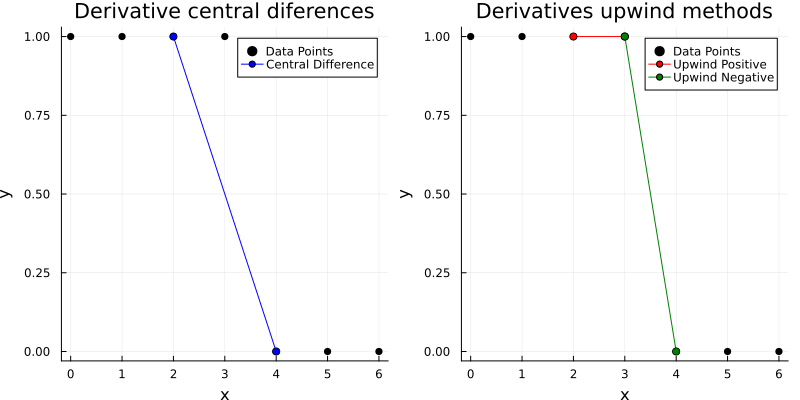
\includegraphics[width=\textwidth]{figures/num_upwind.png}
    \caption{The left figure shows the derivative at point $x=3$ for the central differences method, and the right figure shows the results of the upwind method. The central differences will give a wrong picture if the velocity is positive (moving to the right), because of how the derivative is calculated. For the upwind method we look at different derivatives depending on the direction of the flow. If the flow is positive, we use the red derivative, and if the flow is negative, we use the green derivative.}\label{fig:num_upwind}
\end{figure}

% vind volgende stukken nog leuk maar niet af en dus niet zeker of ik ze wil houden
% Fourier analysis/stability and fourier analysis

% \subsubsection*{stability}
% Another way of seeing the osscilations happen in the central difference scheme is by looking at the effect it has on fourier series. Since we know every smooth enough function is approximable by a fourier series, we can look at the effect of the central difference scheme on a fourier series. Take for example the following fourier series:
% \begin{equation*}
%     u(x) = \sum_{k=-\infty}^{\infty} \hat{u}_k e^{ikx},
% \end{equation*}
% where $\hat{u}_k$ are the fourier coefficients. Now we can look at the effect of the central difference scheme on this fourier series: